\documentclass[../../Aurora C# unofficial manual.tex]{subfiles}

\begin{document}
	\subsection{Automated weapon assignment}
	Original post can be found
	\href{http://aurora2.pentarch.org/index.php?topic=8495.msg107378#msg107378}{here}.
	\\\\
	
	C\# has a more intelligent auto-assignment for weapons and fire controls. You can set up a ship with a single click and then adjust as necessary. The code assumes that:
	\begin{itemize}
		\item Any missile fire control with a resolution of 1 is an anti-missile fire control
		\item Any missile fire control with a resolution greater than 1 is a 'normal' missile fire control
		\item Any beam fire control with a tracking speed at least 2x racial speed is a point defence fire control (some leeway here for older ships)
		\item Other beam fire controls are for offensive weapons
		\item Weapons within the given category (missile PD, missile offensive, beam PD, beam offensive) are split equally between fire controls of the same category
		\item More powerful beam weapons are assigned first
		\item ECCM is assigned as available with the priority order of offensive launcher, PD launcher, offensive beam, PD beam
	\end{itemize}
	
	The assignment code will take account of damage to the ship and adjust accordingly. In most cases, the above will be sufficient (and will be used for NPR designs). For more bespoke and unusual player ships, some tweaking may be necessary.
	
	As a simple example, the escort cruiser below has six twin turrets and three fire controls. Clicking the button assigns two turrets to each fire control and sets the point defence to final fire.
	\begin{figure}[H]
		\centering
		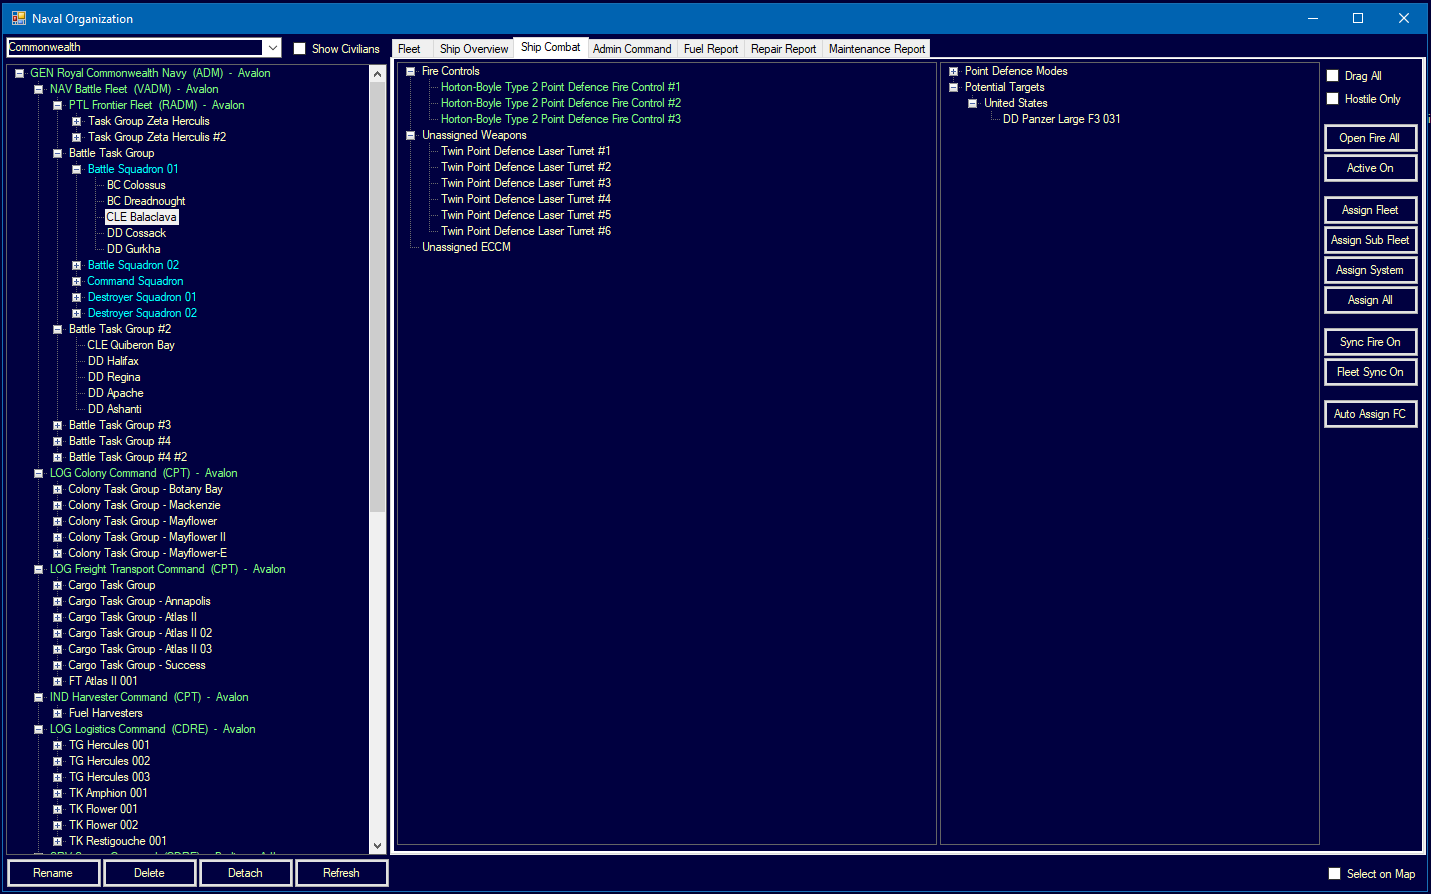
\includegraphics[width=0.95\linewidth]{images/AutomatedAssignment}
		\caption[Automated Assignment]{Automated Assignment Example 1}
		\label{fig:automatedassignment}
	\end{figure}
	\begin{figure}[H]
		\centering
		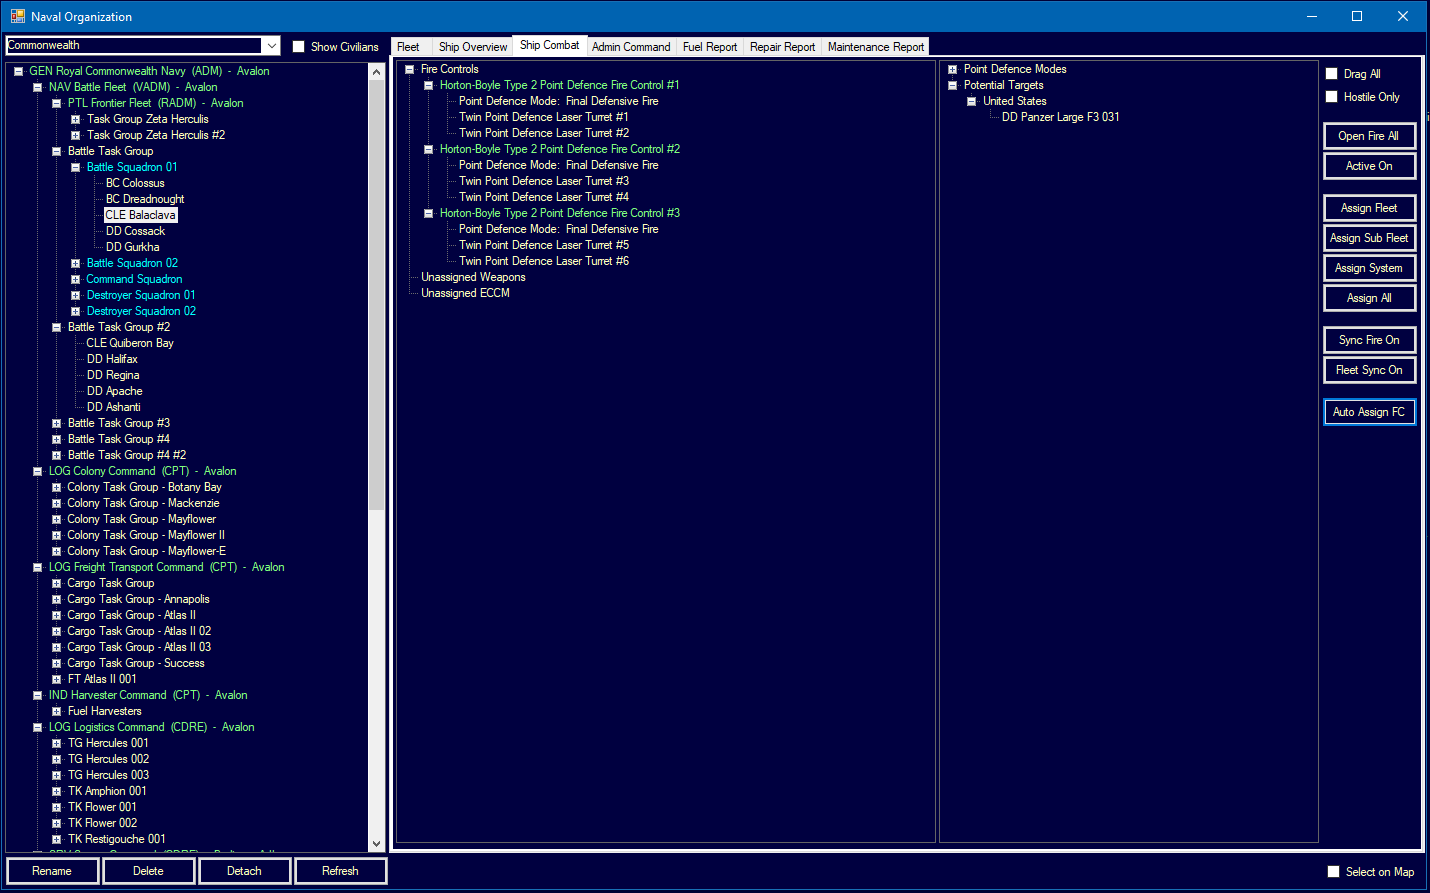
\includegraphics[width=0.95\linewidth]{images/AutomatedAssignment2}
		\caption[Automated Assignment]{Automated Assignment Example 2}
		\label{fig:automatedassignment2}
	\end{figure}
	
	This ship has a mixture of point defence and offensive lasers, plus fire controls for each. The auto-assign determines which weapons should be assigned to which fire control. All beam fire control are set as final fire so the ship will use all available weapons to defend against missile attack.
	\begin{figure}[H]
		\centering
		\begin{subfigure}{.5\textwidth}
			\centering
			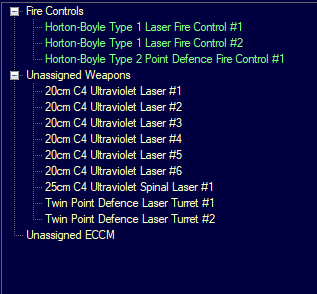
\includegraphics[width=0.5\linewidth]{images/AutomatedAssignment3}
			\caption[Automated Assignment]{Automated Assignment Example 3}
			\label{fig:automatedassignment3}
		\end{subfigure}%
		\begin{subfigure}{.5\textwidth}
			\centering
			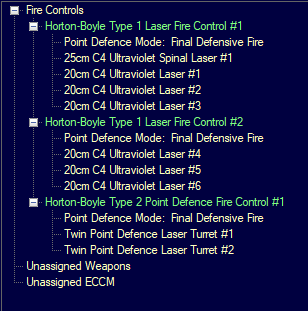
\includegraphics[width=0.5\linewidth]{images/AutomatedAssignment4}
			\caption[Automated Assignment]{Automated Assignment Example 4}
			\label{fig:automatedassignment4}
		\end{subfigure}
	\end{figure}
	
	This ship has a mixture of missiles and offensive lasers. Note that missiles are automatically assigned to launchers.
	\begin{figure}[H]
		\centering
		\begin{subfigure}{.5\textwidth}
			\centering
			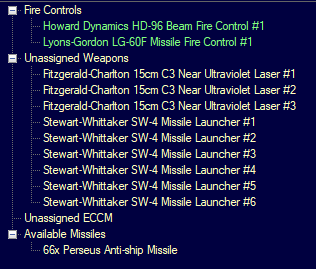
\includegraphics[width=0.5\linewidth]{images/AutomatedAssignment5}
			\caption[Automated Assignment]{Automated Assignment Example 5}
			\label{fig:automatedassignment5}
		\end{subfigure}%
		\begin{subfigure}{.5\textwidth}
			\centering
			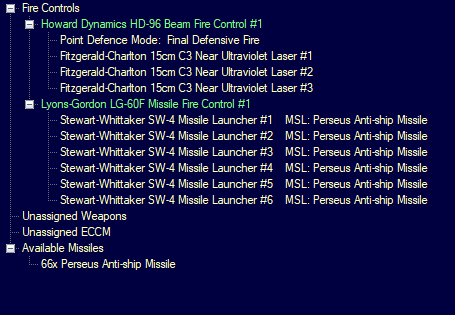
\includegraphics[width=0.5\linewidth]{images/AutomatedAssignment6}
			\caption[Automated Assignment]{Automated Assignment Example 6}
			\label{fig:automatedassignment6}
		\end{subfigure}
	\end{figure}
	
	This ship has a point defence turret and multiple types of offensive beam weapons, plus an ECCM system.
	\begin{figure}[H]
		\centering
		\begin{subfigure}{.5\textwidth}
			\centering
			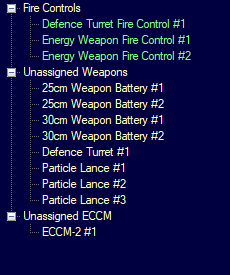
\includegraphics[width=0.5\linewidth]{images/AutomatedAssignment7}
			\caption[Automated Assignment]{Automated Assignment Example 7}
			\label{fig:automatedassignment7}
		\end{subfigure}%
		\begin{subfigure}{.5\textwidth}
			\centering
			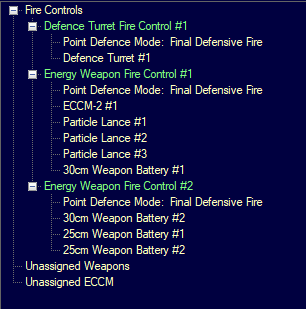
\includegraphics[width=0.5\linewidth]{images/AutomatedAssignment8}
			\caption[Automated Assignment]{Automated Assignment Example 8}
			\label{fig:automatedassignment8}
		\end{subfigure}
	\end{figure}
	
	An extreme example!
	\begin{figure}[H]
		\centering
		\begin{subfigure}{.5\textwidth}
			\centering
			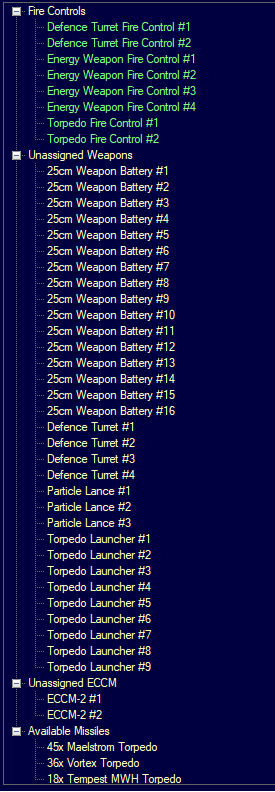
\includegraphics[width=0.5\linewidth]{images/AutomatedAssignment9}
			\caption[Automated Assignment]{Automated Assignment Example 9}
			\label{fig:automatedassignment9}
		\end{subfigure}%
		\begin{subfigure}{.5\textwidth}
			\centering
			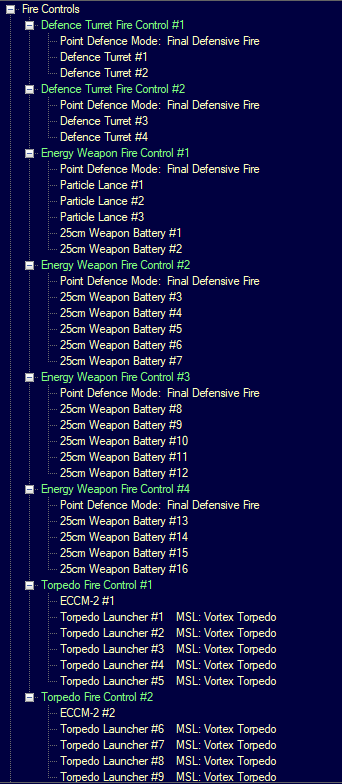
\includegraphics[width=0.5\linewidth]{images/AutomatedAssignment10}
			\caption[Automated Assignment]{Automated Assignment Example 10}
			\label{fig:automatedassignment10}
		\end{subfigure}
	\end{figure}
\end{document}